\chapter{Adaptations des plantes et plasticité phénotypique}\label{ch:b2:plant-plasticity}

Deux feuilles d'un même chêne~: celle du sommet de la couronne est
petite, épaisse et coriace, celle de l'intérieur ombragé trois fois plus
grande et fine comme du papier. Une plantule de ce même chêne sous un
couvert fermé pousse haute et grêle~; sa sœur dans une clairière reste
courte et trapue. Aucune de ces différences n'est génétique. Une plante
ne peut pas marcher vers un meilleur endroit~; elle se construit donc à
la mesure de l'endroit où elle se trouve~: elle perçoit la lumière, la
gravité, le contact, l'eau, le sel, le froid, et en conséquence elle se
courbe, s'épaissit, s'allonge, ferme ses pores ou endurcit ses
cellules. Ce chapitre traite de cette plasticité --- la manière dont une
plante lit son environnement et ce qu'elle en fait --- et des
\omterm{def:b2:plant-plasticity:plasticity}{adaptations} héréditaires par lesquelles des lignées se sont ajustées
aux déserts, à l'ombre, au sel et au gel.

\section{La plasticité et ses limites}

\begin{definition}[Plasticité phénotypique et norme de réaction]\label{def:b2:plant-plasticity:plasticity}
\index{plasticite phenotypique@plasticité phénotypique}\index{norme de reaction@norme de réaction}\index{acclimatation}\index{adaptation}
La \emph{plasticité phénotypique} est la capacité d'un même \omterm{def:b2:meiosis-heredity:vocabulary}{génotype} à
produire des \omterm{def:b2:meiosis-heredity:vocabulary}{phénotypes} différents dans des environnements différents.
La \emph{norme de réaction} d'un \omterm{def:b2:meiosis-heredity:vocabulary}{génotype} est la courbe de son \omterm{def:b2:meiosis-heredity:vocabulary}{phénotype}
en fonction d'une variable de l'environnement --- l'épaisseur des
feuilles en fonction de la lumière, la longueur de la tige en fonction
de la température~; les \omterm{def:b2:meiosis-heredity:vocabulary}{génotypes} diffèrent par leurs normes, et ces
différences sont héréditaires, même lorsque la réponse plastique
elle-même ne l'est pas. L'\emph{acclimatation} en est la forme
physiologique et réversible~: une feuille qui épaissit sa cuticule
pendant une semaine sèche, une cellule qui fabrique un antigel en
automne. L'\emph{adaptation}, au sens évolutif, est l'ajustement
héréditaire d'une lignée à son habitat, sélectionné au fil des
générations~: un cactus est adapté à la sécheresse, un haricot
s'acclimate à une période sèche. Les plantes sont plus plastiques que
les animaux parce qu'elles sont modulaires et à croissance indéfinie
(\cref{ch:b2:plant-meristems})~: la feuille suivante peut être
construite autrement que la précédente, et la vie fixée fait de la
plasticité la seule manière de se déplacer.
\end{definition}

\begin{omfigure}
\begin{tikzpicture}
\begin{axis}[
  width=0.72\linewidth, height=5.4cm,
  axis x line=bottom, axis y line=left,
  xmin=0, xmax=100, ymin=0, ymax=1.2,
  xlabel={lumière (\% du plein soleil)}, ylabel={épaisseur des feuilles (relative)},
  xlabel style={font=\small, at={(axis description cs:0.5,-0.13)}, anchor=north},
  ylabel style={font=\small},
  tick label style={font=\small}, xtick={0,25,50,75,100}, ytick={0,0.5,1},
  legend style={font=\scriptsize, at={(0.97,0.08)}, anchor=south east, draw=none},
  clip=false,
]
\addplot[very thick, omDef, domain=2:100, samples=60] {0.35 + 0.65*(1-exp(-x/30))};
\addlegendentry{génotype 1~: un chêne plastique}
\addplot[very thick, omThm, domain=2:100, samples=60] {0.55 + 0.2*(1-exp(-x/30))};
\addlegendentry{génotype 2~: un chêne moins plastique}
\end{axis}
\end{tikzpicture}

{\small Deux \omterm{def:b2:plant-plasticity:plasticity}{normes de réaction}. Chaque \omterm{def:b2:meiosis-heredity:vocabulary}{génotype} produit des feuilles
plus épaisses sous une lumière plus forte~; la pente de la courbe --- la
plasticité --- est elle-même un caractère héréditaire, et les deux
\omterm{def:b2:meiosis-heredity:vocabulary}{génotypes} diffèrent par ce caractère.}
\end{omfigure}

\begin{proposition}[Feuilles de lumière et feuilles d'ombre]\label{prop:b2:plant-plasticity:sunshade}
\index{feuille de lumiere@feuille de lumière}\index{feuille d'ombre}
Une feuille qui se développe en plein soleil est petite et épaisse,
avec deux ou trois assises de cellules palissadiques, de nombreux
stomates, une cuticule épaisse, une forte concentration de l'enzyme de
fixation du carbone et une vitesse maximale de photosynthèse élevée~;
une feuille de la même plante qui se développe à l'ombre est grande et
fine, avec une seule assise palissadique, plus de chlorophylle par unité
de masse, une faible respiration et un point de compensation lumineux
bas. La \omterm{prop:b2:plant-plasticity:sunshade}{feuille d'ombre} est construite pour récolter chaque photon à
moindre coût, la \omterm{prop:b2:plant-plasticity:sunshade}{feuille de lumière} pour exploiter un flot de photons
sans surchauffer ni flétrir. La décision est prise alors que la feuille
n'est encore qu'un primordium, d'après la lumière --- et en particulier
sa couleur --- qui atteint le bourgeon~; une feuille mûre ne peut pas se
reconstruire, et c'est pourquoi une plante déplacée de l'ombre au soleil
brûle jusqu'à ce qu'elle ait produit de nouvelles feuilles.
\end{proposition}

\begin{omfigure}
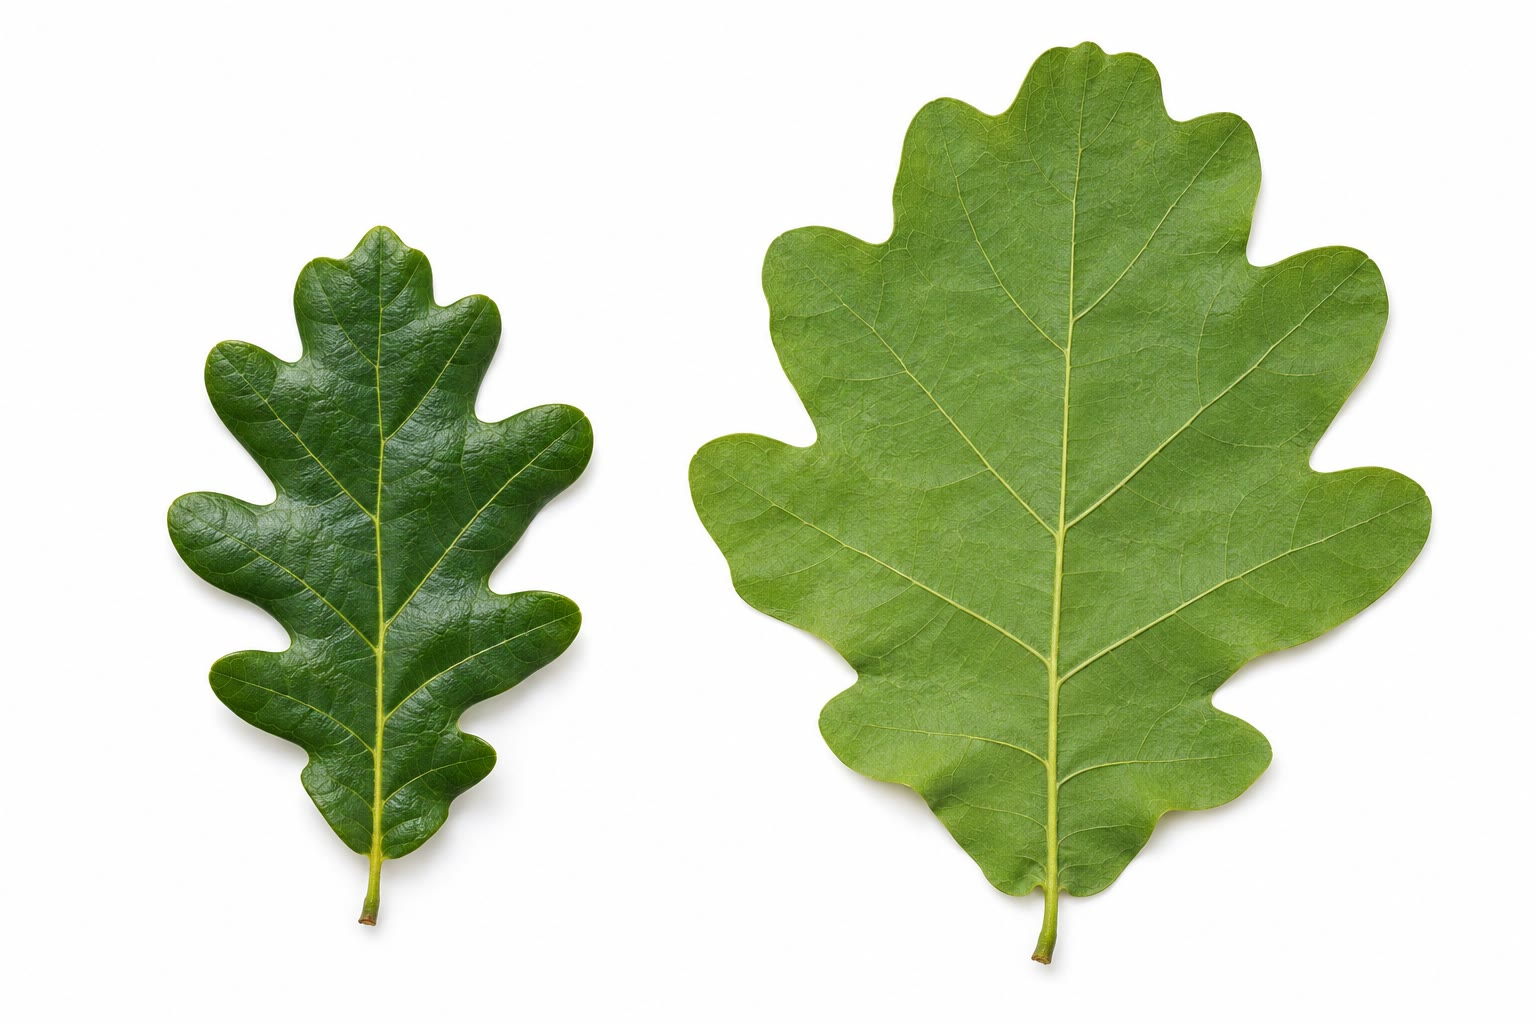
\includegraphics[width=0.55\linewidth]{images/book4/ai/b4-15-sun-shade-leaves.jpg}

{\small Une \omterm{prop:b2:plant-plasticity:sunshade}{feuille de lumière} et une \omterm{prop:b2:plant-plasticity:sunshade}{feuille d'ombre} d'un même chêne~:
même \omterm{def:b2:meiosis-heredity:vocabulary}{génotype}, lumière différente, feuilles différentes.}
\end{omfigure}

\section{Lire la lumière}

\begin{theorem}[Le phytochrome, mesureur de la qualité de la lumière]\label{thm:b2:plant-plasticity:phytochrome}
\index{phytochrome}\index{rapport rouge/rouge lointain}\index{evitement de l'ombre@évitement de l'ombre}
Le phytochrome existe sous deux formes~: $P_r$, qui absorbe la lumière
rouge (\qty{660}{nm}) et se convertit en $P_{fr}$, et $P_{fr}$, qui
absorbe le rouge lointain (\qty{730}{nm}) et se reconvertit --- et c'est
$P_{fr}$ qui agit. En lumière continue, les deux conversions
s'équilibrent en un \emph{photoéquilibre} dont la position ne dépend que
du rapport du rouge au rouge lointain dans la lumière~:
\[
\varphi = \frac{P_{fr}}{P_{r} + P_{fr}} = \frac{R}{R + a\,FR},
\]
où $R$ et $FR$ sont les densités de flux de photons dans les deux bandes
et $a$ une constante du pigment ($a \approx 0.77$). La lumière solaire a
$R{:}FR \approx 1.15$, ce qui donne $\varphi \approx 0.6$~; la lumière
filtrée par les feuilles, qui absorbent le rouge et transmettent le rouge
lointain, a $R{:}FR
\approx 0.2$ et $\varphi \approx 0.2$. Un $\varphi$ faible indique à une
plante qu'elle se trouve sous d'autres plantes ou à côté d'elles avant
même d'être réellement ombragée --- le rouge lointain réfléchi par une
voisine est détecté sur la face tournée vers elle --- et elle répond par
le \emph{syndrome d'\omterm{thm:b2:plant-plasticity:phytochrome}{évitement de l'ombre}}~: allongement plus rapide de
la tige, pétioles plus longs, feuilles redressées, ramification réduite,
floraison plus précoce. Une plantule sous un couvert fermé double sa
vitesse d'allongement.
\end{theorem}
\begin{proof}
Soit $k_1 R$ la constante de vitesse de $P_r \to P_{fr}$ (proportionnelle
au flux rouge) et $k_2\,FR$ celle de $P_{fr} \to P_r$. À l'équilibre,
$k_1 R\,P_r = k_2\,FR\,P_{fr}$, donc $P_{fr}/P_r = k_1 R/
(k_2 FR)$ et $\varphi = P_{fr}/(P_r + P_{fr}) = R/(R + a\,FR)$ avec
$a = k_2/k_1$. (Les deux formes absorbent un peu dans les deux bandes,
ce qu'intègre la constante $a$~; la forme du résultat est inchangée.)
Avec $a = 0.77$~: $1.15/(1.15 + 0.77) = 0.60$~; $0.2/(0.2 + 0.77) = 0.21$.
\end{proof}

\begin{omfigure}
\begin{tikzpicture}
\begin{axis}[
  width=0.7\linewidth, height=5.2cm,
  axis x line=bottom, axis y line=left,
  xmin=0, xmax=1.4, ymin=0, ymax=0.8,
  xlabel={rapport rouge : rouge lointain de la lumière}, ylabel={$\varphi = P_{fr}/P_{\text{total}}$},
  xlabel style={font=\small, at={(axis description cs:0.5,-0.13)}, anchor=north},
  ylabel style={font=\small},
  tick label style={font=\small}, xtick={0,0.2,0.6,1.15}, ytick={0,0.2,0.4,0.6},
  clip=false,
]
\addplot[very thick, omDef, domain=0:1.4, samples=60] {x/(x+0.77)};
\draw[dashed, gray] (axis cs:1.15,0) -- (axis cs:1.15,0.6) -- (axis cs:0,0.6); \node[font=\scriptsize, anchor=south west] at (axis cs:1.15,0.6) {plein soleil};
\draw[dashed, gray] (axis cs:0.2,0) -- (axis cs:0.2,0.21) -- (axis cs:0,0.21); \node[font=\scriptsize, anchor=west] at (axis cs:0.25,0.15) {sous un couvert};
\end{axis}
\end{tikzpicture}

{\small Le photoéquilibre du phytochrome en fonction du \omterm{thm:b2:plant-plasticity:phytochrome}{rapport rouge/rouge
lointain}. La lumière solaire maintient la plus grande partie du pigment
sous forme active~; la lumière filtrée par les feuilles le maintient
surtout inactif, et la plante interprète la différence comme la
présence de voisines.}
\end{omfigure}

\begin{proposition}[Le phototropisme]\label{prop:b2:plant-plasticity:phototropism}
\index{phototropisme}\index{tropisme}\index{hypothese de Cholodny--Went@hypothèse de Cholodny--Went}
Un \emph{tropisme} est un mouvement de croissance orienté par un
stimulus directionnel. Dans le \emph{phototropisme}, une pousse se
courbe vers la lumière bleue~: la lumière est perçue à l'extrémité par
un récepteur de la lumière bleue (la phototropine), l'auxine qui
descend de l'extrémité est redirigée vers la face ombragée --- ses
transporteurs gagnent la membrane latérale --- et la face ombragée,
recevant plus d'auxine, s'allonge plus vite que la face éclairée, si
bien que la pousse se courbe vers la lumière. La courbure est une
croissance différentielle, non l'action d'un muscle~: elle ne se produit
que dans la \omterm{prop:b2:plant-meristems:ram}{zone d'élongation}, prend une heure ou deux et est
irréversible. Les racines, chez lesquelles le même excès d'auxine
\emph{inhibe} l'allongement, se courbent en sens inverse.
\end{proposition}
\begin{proof}[Faits expérimentaux]
Darwin (1880) montra, sur des coléoptiles de graminées, que l'extrémité
perçoit la lumière et que la zone située en dessous se courbe~:
recouvrir l'extrémité d'un capuchon opaque supprimait la courbure,
recouvrir la base d'un tube ne la supprimait pas, et un capuchon
transparent la laissait intacte. Boysen-Jensen (1913) coupa l'extrémité
et la replaça en intercalant un bloc de gélatine~: la courbure
persistait, le signal était donc une substance diffusible~; une lame de
mica insérée du côté ombragé la bloquait, du côté éclairé non~: la
substance descendait donc par la face ombragée. Went (1928) recueillit
la substance dans de la gélose à partir d'extrémités coupées et
constata qu'un bloc posé de façon excentrée sur un coléoptile décapité,
à l'obscurité, le faisait se courber du côté opposé au bloc --- d'un
angle proportionnel à la quantité --- et, en recueillant la gélose sous
les deux moitiés d'une extrémité éclairée d'un seul côté, trouva
environ deux tiers de l'auxine du côté ombragé et un tiers du côté
éclairé (Briggs, 1957, avec de meilleures méthodes). La redistribution
latérale d'une hormone de croissance constitue l'\omterm{prop:b2:plant-plasticity:phototropism}{hypothèse de
Cholodny--Went}, et elle a résisté.
\end{proof}

\begin{omfigure}
\begin{tikzpicture}[every node/.style={font=\scriptsize}, >=stealth]
  \foreach \x/\lab/\cap/\bend in {0/{intact~:\\courbure}/0/1, 2.6/{extrémité couverte~:\\pas de courbure}/1/0, 5.2/{base couverte~:\\courbure}/2/1, 7.8/{extrémité coupée~:\\pas de courbure}/3/0, 10.4/{extrémité sur gélatine~:\\courbure}/4/1} {
    \begin{scope}[xshift=\x cm]
      \fill[omExo!30] (-0.7,0) rectangle (0.7,0.2);
      \ifnum\bend=1
        \draw[very thick, omExo!70!black] (0,0.2) -- (0,1.6) .. controls (0,2.3) and (0.5,2.6) .. (0.9,2.8);
      \else
        \draw[very thick, omExo!70!black] (0,0.2) -- (0,3.0);
      \fi
      \ifnum\cap=1 \fill[black] (-0.2,2.7) rectangle (0.2,3.1); \fi
      \ifnum\cap=2 \fill[black] (-0.2,0.2) rectangle (0.2,1.5); \fi
      \ifnum\cap=3 \draw[thick] (-0.3,2.6) -- (0.3,2.6); \fi
      \ifnum\cap=4 \fill[omDef!35] (-0.2,2.55) rectangle (0.2,2.75); \draw[very thick, omExo!70!black] (0.55,2.75) -- (0.9,3.1); \fi
      \node[below, align=center] at (0,-0.15) {\lab};
    \end{scope}
  }
  \node[anchor=east, align=right, omProp!80!black] at (-1.0,2.2) {lumière venant\\de la droite $\to$};
\end{tikzpicture}

{\small Les expériences sur le coléoptile. Darwin~: l'extrémité perçoit
la lumière et la région située en dessous se courbe~; coiffer
l'extrémité empêche la courbure, protéger la base ne l'empêche pas.
Boysen-Jensen~: le signal traverse un bloc de gélatine --- c'est une
substance.}
\end{omfigure}

\begin{omfigure}
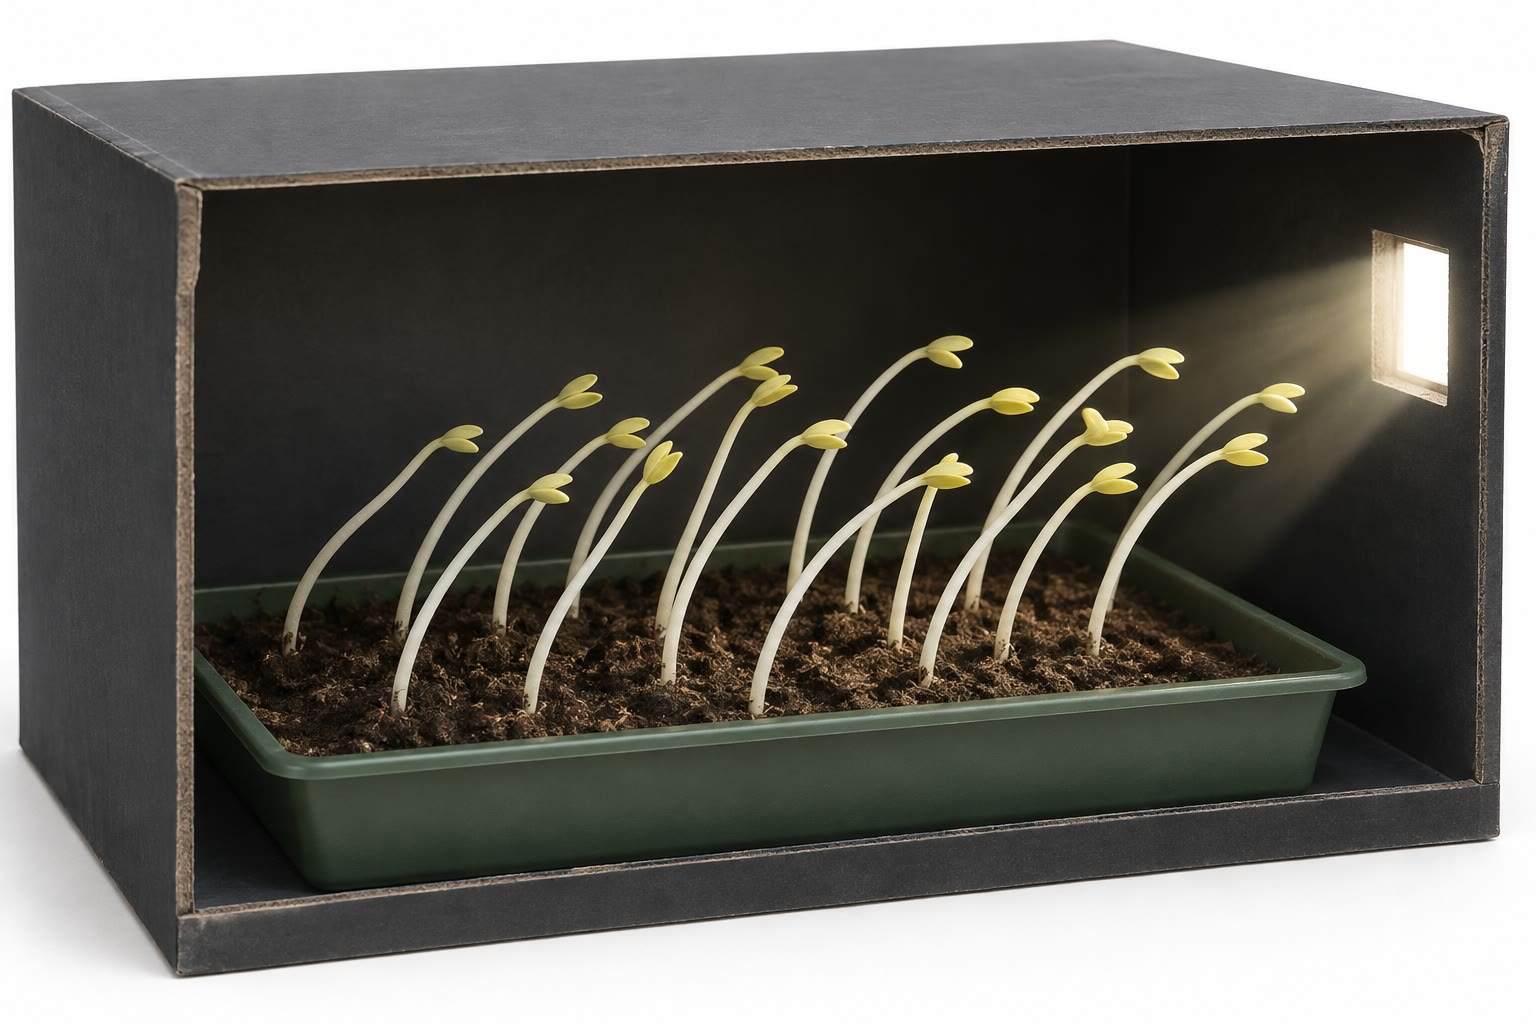
\includegraphics[width=0.55\linewidth]{images/book4/ai/b4-15-phototropism.jpg}

{\small Des plantules dans une boîte à une seule fenêtre~: toutes se
courbent vers la lumière, en croissant plus vite du côté opposé.}
\end{omfigure}

\begin{theorem}[De combien une tige se courbe]\label{thm:b2:plant-plasticity:bend}
Si la face ombragée d'une tige de diamètre $d$ s'allonge d'une quantité
relative $\varepsilon_s$ et la face éclairée de $\varepsilon_l$ sur une
zone de croissance de longueur $L$, la zone se courbe d'un angle
\[
\theta = \frac{L\,(\varepsilon_s - \varepsilon_l)}{d}
\]
(en radians). Un coléoptile qui croît de \qty{5}{\%} par heure sur une
zone de \qty{10}{mm} de long et de \qty{1}{mm} de diamètre, avec une
auxine répartie selon
$65 : 35$, si bien que les deux faces croissent à $1.3$ et $0.7$ fois
la vitesse moyenne, se courbe en trois heures de
$\theta = 10\times(0.195 - 0.105)/1 =
0.9$ radian, soit environ \qty{50}{\degree}. La courbure n'exige aucun
mécanisme nouveau~: la croissance ordinaire du
\cref{ch:b2:plant-meristems}, rendue inégale sur deux faces, suffit.
\end{theorem}
\begin{proof}
Les deux faces de la zone deviennent des arcs de rayons $\rho + d/2$ et
$\rho - d/2$ qui sous-tendent le même angle $\theta$, de longueurs $L(1 +
\varepsilon_s)$ et $L(1 + \varepsilon_l)$~; leur différence vaut
$\theta d$, donc $\theta = L(\varepsilon_s - \varepsilon_l)/d$. En trois
heures à \qty{5}{\%} par heure, l'extension moyenne vaut $0.15$~;
$1.3\times 0.15 = 0.195$ et $0.7\times 0.15 = 0.105$.
\end{proof}

\begin{proposition}[Le gravitropisme]\label{prop:b2:plant-plasticity:gravitropism}
\index{gravitropisme}\index{statolithe}
Une pousse couchée sur le côté se redresse vers le haut, et une racine
se tourne vers le bas, en quelques heures. La direction de la gravité
est perçue par des \emph{statolithes} --- des grains d'amidon denses
situés dans des cellules spécialisées de la coiffe racinaire et de
l'endoderme amylifère de la tige --- qui sédimentent en quelques secondes
sur la face inférieure de la cellule et, en appuyant sur la membrane ou
sur le réticulum endoplasmique, redirigent les transporteurs d'auxine,
si bien que l'auxine s'accumule sur la face inférieure. Dans la pousse,
la face inférieure croît plus vite et la tige se courbe vers le haut~;
dans la racine, le même excès d'auxine inhibe la face inférieure, la
face supérieure croît plus vite et la racine se courbe vers le bas. Si
l'on retire la coiffe, la racine croît droit dans n'importe quelle
direction~; les mutants dépourvus d'amidon perçoivent mal la gravité~;
une racine placée sur un tambour en lente rotation (un clinostat), qui
ne laisse jamais les statolithes sédimenter, croît sans direction. La
réponse est une seconde utilisation du mécanisme de Cholodny--Went, avec
un capteur différent.
\end{proposition}

\section{L'eau~: fermer les pores}

\begin{proposition}[Le contrôle stomatique]\label{prop:b2:plant-plasticity:stomata}
\index{stomate}\index{cellule de garde}\index{acide abscissique}\index{conductance stomatique}
Les pores de la feuille, les \emph{stomates}, sont chacun bordés de deux
\emph{\omterm{prop:b2:plant-plasticity:stomata}{cellules de garde}} dont les parois sont inégalement épaissies~:
lorsqu'elles absorbent du potassium et de l'eau et gonflent, elles
s'incurvent et ouvrent le pore, et lorsqu'elles les perdent, elles le
ferment. Ils s'ouvrent le matin sous l'effet de la lumière bleue et
d'une faible concentration interne de $\mathrm{CO_2}$, et se ferment à
l'obscurité~; ils se ferment en quelques minutes à l'arrivée d'\emph{\omterm{def:b2:plant-flowering:dormancy}{acide
abscissique}} --- produit par des racines qui perçoivent l'assèchement du
sol et transporté vers le haut dans le xylème, ou produit dans la feuille
elle-même lorsqu'elle perd sa turgescence --- et lorsque l'air est très
sec. La \emph{\omterm{prop:b2:plant-plasticity:stomata}{conductance stomatique}} $g_s$ fixe à la fois l'eau perdue,
$E = g_s\,(w_i - w_a)$ (la différence de fraction molaire de vapeur d'eau
entre l'intérieur de la feuille, saturé, et l'air), et le
$\mathrm{CO_2}$ absorbé, $A = g_s\,(c_a -
c_i)/1.6$ (le facteur $1.6$ étant le rapport des diffusivités de la
vapeur d'eau et du $\mathrm{CO_2}$). La feuille échange de l'eau contre
du carbone par une seule soupape, et son \emph{efficience d'utilisation
de l'eau} vaut
\[
\frac{A}{E} = \frac{c_a - c_i}{1.6\,(w_i - w_a)},
\]
quelques millièmes de mole de carbone par mole d'eau~: une feuille
C$_3$ typique dépense \qtyrange{400}{600}{g} d'eau par gramme de carbone
fixé, une feuille C$_4$ la moitié, une \omterm{prop:b2:plant-plasticity:xerophytes}{plante CAM} le cinquième.
\end{proposition}

\begin{omfigure}
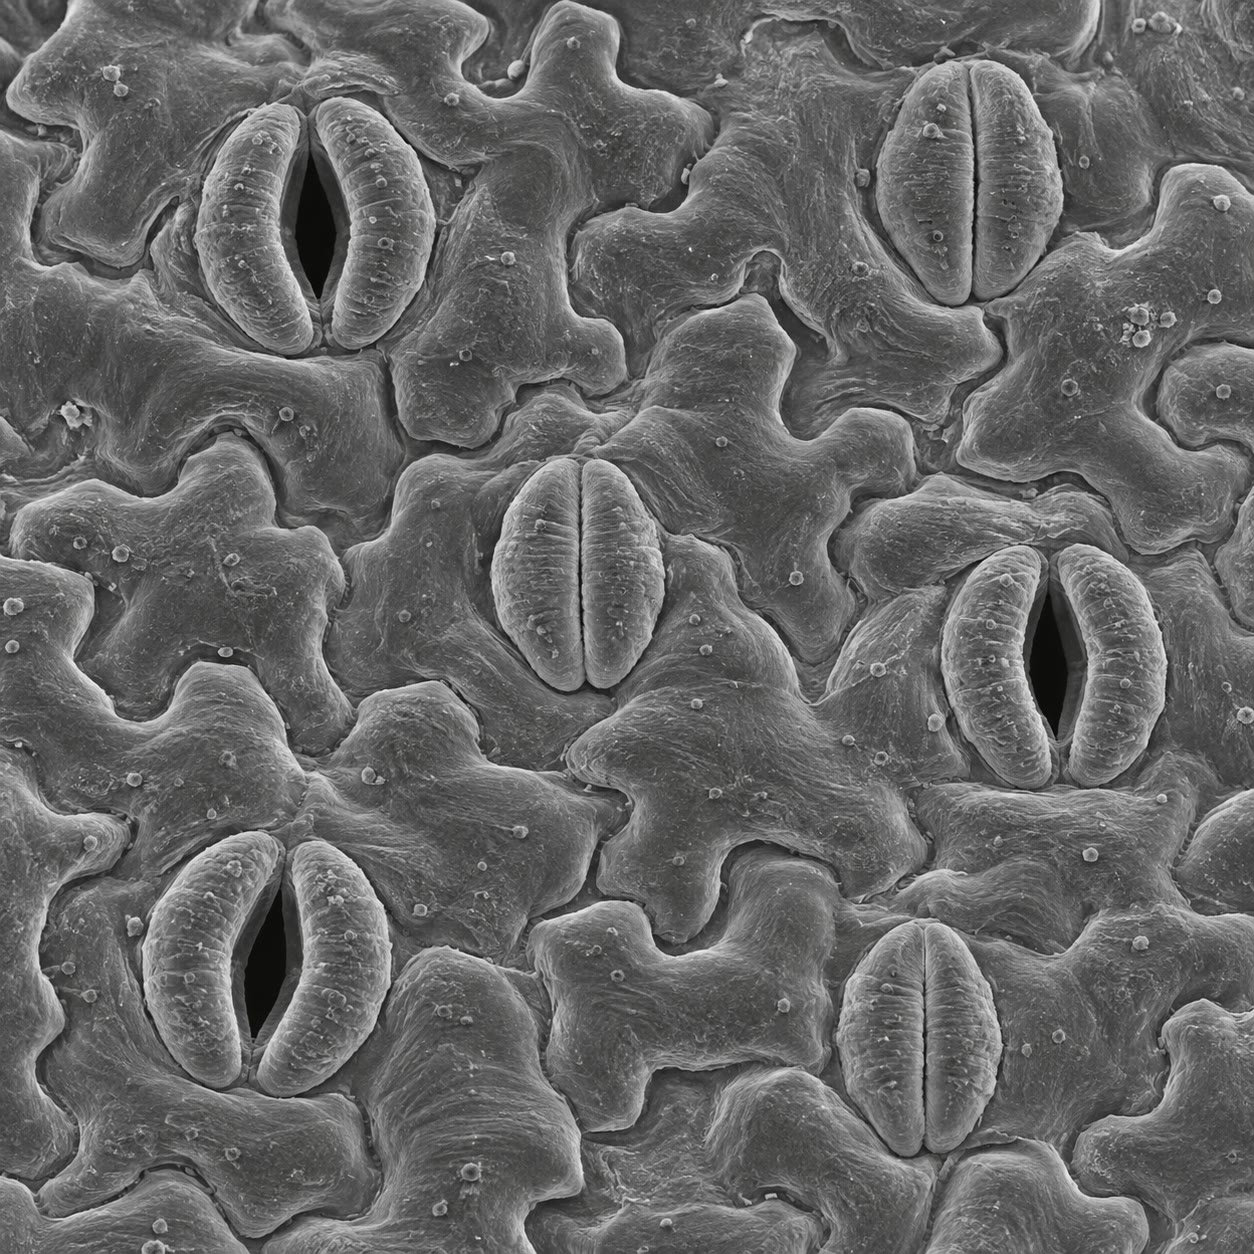
\includegraphics[width=0.42\linewidth]{images/book4/ai/b4-15-stomata-sem.jpg}

{\small Des stomates sur la face inférieure d'une feuille, certains
ouverts, d'autres fermés~: deux \omterm{prop:b2:plant-plasticity:stomata}{cellules de garde} autour de chaque pore,
la soupape par laquelle la feuille échange de l'eau contre du dioxyde de
carbone.}
\end{omfigure}

\begin{example}[Le coût du carbone d'une journée]\label{ex:b2:plant-plasticity:wue}
À midi, une feuille de tournesol avec $g_s = \qty{0.3}{mol.m^{-2}.s^{-1}}$,
$w_i - w_a = 0.02$ et $c_a - c_i = \qty{120}{\micro mol/mol}$ transpire
$E = \qty{6}{mmol.m^{-2}.s^{-1}}$ et fixe $A =
0.3\times 120/1.6 = \qty{22}{\micro mol.m^{-2}.s^{-1}}$~: $A/E =
\qty{3.7e-3}{}$, c'est-à-dire 270 molécules d'eau par atome de carbone,
\qty{400}{g} d'eau par gramme de carbone. Un hectare de telles feuilles
perd \qty{40}{t} d'eau par jour d'été pour fixer \qty{100}{kg} de
carbone. Lorsque le sol s'assèche, l'\omterm{def:b2:plant-flowering:dormancy}{acide abscissique} réduit la
conductance des stomates au dixième de cette valeur~: $E$ est divisé par
dix, $A$ moins que cela (puisque $c_i$ diminue aussi), et la plante
survit à la diète plutôt que de mourir de soif.
\end{example}

\begin{proposition}[Les adaptations à la sécheresse]\label{prop:b2:plant-plasticity:xerophytes}
\index{xerophyte@xérophyte}\index{plante CAM}\index{plante succulente}
Les plantes des milieux secs (\emph{xérophytes}) associent des
structures et des stratégies héréditaires. Réduire les pertes~: cuticule
épaisse, stomates enfoncés dans des cryptes ou cachés sous des poils (qui
épaississent la couche d'air immobile), feuilles réduites à des épines
(cactus) ou tombant à la saison sèche, petites feuilles épaisses qui
s'enroulent. Stocker~: tiges et feuilles succulentes, riches en mucilage
qui retient l'eau. Atteindre l'eau~: racines profondes de \qty{50}{m}
(prosopis) ou étalées juste sous la surface pour capter une averse.
Décaler~: les \omterm{prop:b2:plant-plasticity:xerophytes}{plantes CAM} ouvrent leurs stomates la nuit, lorsque
$w_i - w_a$ est faible, fixent le
$\mathrm{CO_2}$ sous forme d'acide malique, et le refixent le jour,
stomates fermés --- le même carbone pour le cinquième de l'eau.
Échapper~: les annuelles du désert vivent sous forme de \omterm{def:b2:angiosperm-reproduction:seed}{graines} pendant
des années et accomplissent leur \omterm{def:b2:plant-life-cycles:cycles}{cycle de vie} dans les semaines qui
suivent la pluie. Tolérer~: les plantes reviviscentes perdent
\qty{95}{\%} de leur eau et reviennent à la vie. Chaque stratégie a un
prix --- le métabolisme CAM est lent, la succulence est lourde, les
épines ne font pas la photosynthèse --- et la plante qui le paie est
supplantée partout où l'eau est abondante.
\end{proposition}

\begin{omfigure}
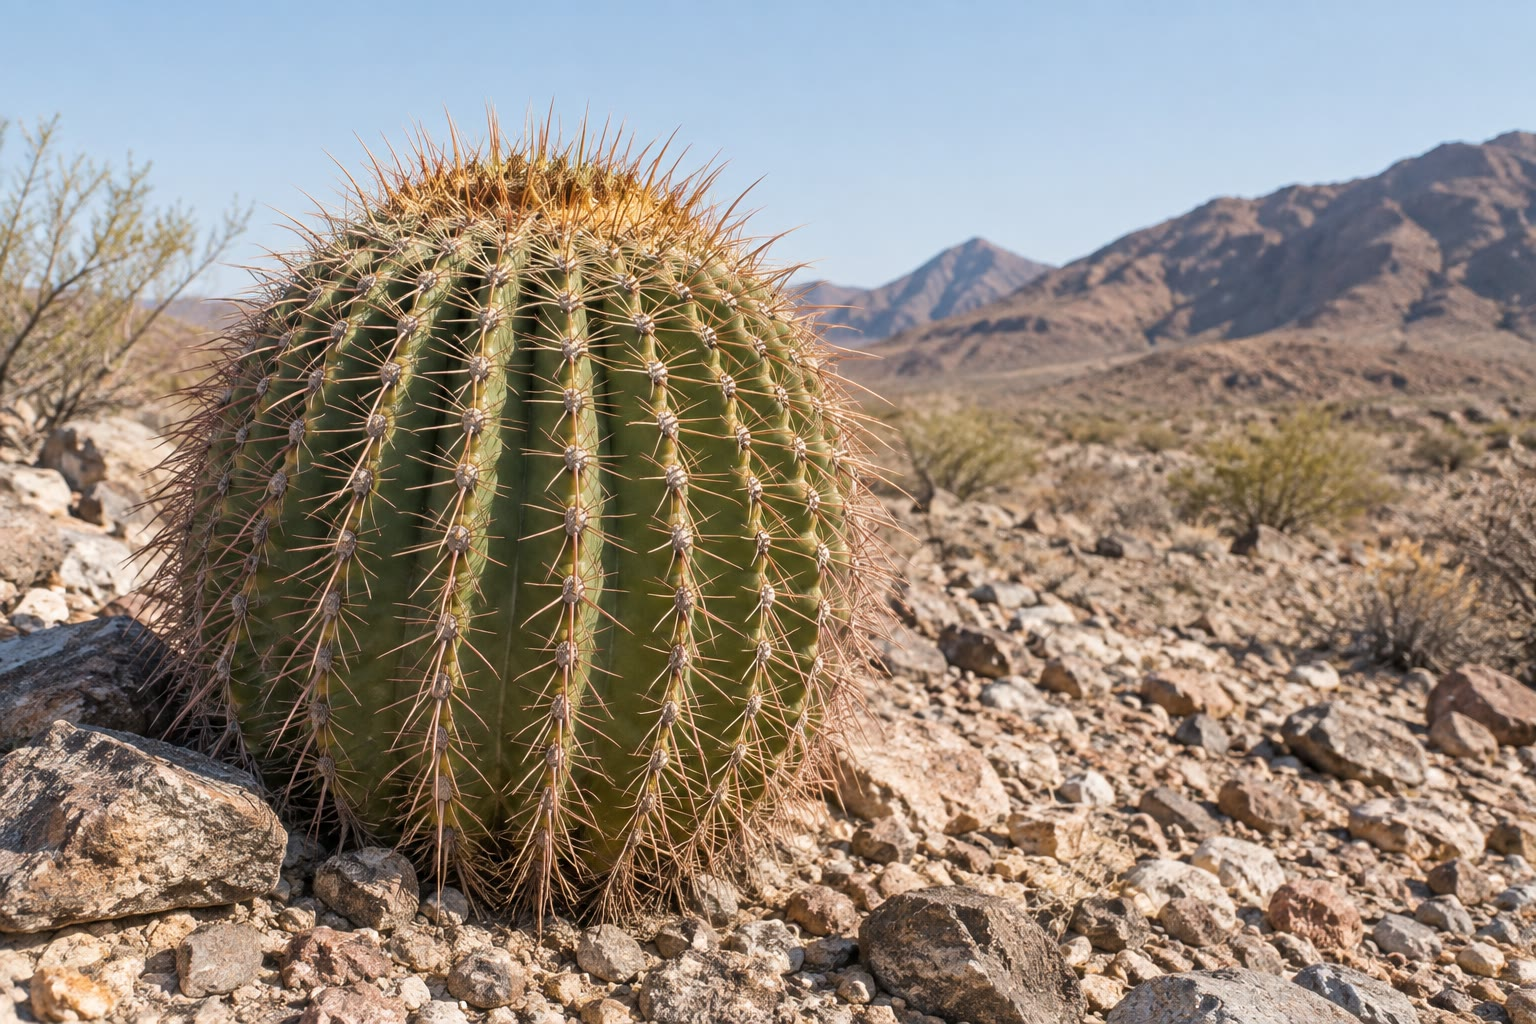
\includegraphics[width=0.55\linewidth]{images/book4/ai/b4-15-cactus.jpg}

{\small Un cactus en tonneau~: une tige succulente à cuticule épaisse,
des côtes qui lui permettent de gonfler après la pluie, des feuilles
réduites à des épines, et des stomates qui ne s'ouvrent que la nuit.}
\end{omfigure}

\section{Froid, sel et réponse au stress}

\begin{proposition}[L'acclimatation au stress]\label{prop:b2:plant-plasticity:stress}
\index{acclimatation au froid}\index{halophyte}\index{proteine de choc thermique@protéine de choc thermique}
Une semaine à \qty{4}{\celsius} abaisse la température létale d'un
seigle d'hiver de \qty{-5}{\celsius} à \qty{-25}{\celsius}~: les
cellules ont accumulé des sucres et des protéines qui abaissent le point
de congélation et protègent les membranes, modifié leurs lipides pour
qu'ils restent fluides, et fabriqué des protéines antigel qui empêchent
la croissance des cristaux de glace~; l'événement létal n'est pas la
glace, qui se forme sans dommage entre les cellules, mais la
déshydratation de la cellule lorsque l'eau la quitte pour rejoindre la
glace. Quelques heures à \qty{40}{\celsius} induisent des
\emph{\omterm{prop:b2:plant-plasticity:stress}{protéines de choc thermique}} qui replient les protéines dénaturées
et protègent la cellule à \qty{45}{\celsius}. Face au sel, la plante
recourt à l'exclusion au niveau des racines, au stockage dans la
vacuole (avec des solutés compatibles dans le cytosol pour
l'équilibrer) et, chez les véritables \emph{halophytes}, à la sécrétion
par des glandes à sel. La plupart de ces réponses empruntent la même
signalisation~: un capteur, une hausse du calcium cytosolique, l'\omterm{def:b2:plant-flowering:dormancy}{acide
abscissique}, et un ensemble de \omterm{prop:b2:cell-differentiation:transcriptional}{facteurs de transcription} qui activent
des centaines de gènes protecteurs --- un programme de stress aussi
général que la réponse immunitaire d'un animal et, comme elle, coûteux~:
la plante acclimatée croît lentement, et une plante qui s'acclimate sans
nécessité est supplantée par une plante qui ne le fait pas.
\end{proposition}
\begin{proof}[Faits expérimentaux]
Les expériences d'\omterm{prop:b2:plant-plasticity:stress}{acclimatation au froid} mesurent la température à
laquelle meurent la moitié des cellules d'une feuille (la LT$_{50}$)
avant et après une période à basse température~; le décalage, de dix à
vingt degrés en une semaine, est annulé par une semaine de chaleur. Les
mutants incapables d'activer le programme du froid (les \omterm{prop:b2:cell-differentiation:transcriptional}{facteurs de
transcription} CBF) s'acclimatent mal, et les plantes qui expriment ces
facteurs de façon constitutive survivent au gel sans \omterm{def:b2:plant-plasticity:plasticity}{acclimatation} ---
mais restent naines.
\end{proof}

\begin{omfigure}
\begin{tikzpicture}[every node/.style={font=\scriptsize}, >=stealth]
  \node[draw, rounded corners, fill=omExo!25, align=center] (s) at (0,0) {stress\\sécheresse, froid,\\sel, chaleur};
  \node[draw, rounded corners, fill=omDef!15, align=center] (sen) at (3.2,0) {capteur\\(membrane, turgescence,\\protéines dépliées)};
  \node[draw, rounded corners, fill=omDef!15, align=center] (ca) at (6.4,0) {seconds messagers\\Ca$^{2+}$, ABA};
  \node[draw, rounded corners, fill=omProp!20, align=center] (tf) at (9.6,0) {facteurs de\\transcription};
  \node[draw, rounded corners, fill=omThm!15, align=center] (out) at (12.8,0.9) {gènes protecteurs~:\\solutés, antigel,\\chaperons, transporteurs};
  \node[draw, rounded corners, fill=omThm!15, align=center] (out2) at (12.8,-0.9) {croissance ralentie~:\\le coût};
  \draw[->, thick] (s) -- (sen); \draw[->, thick] (sen) -- (ca); \draw[->, thick] (ca) -- (tf);
  \draw[->, thick] (tf) -- (out); \draw[->, thick] (tf) -- (out2);
\end{tikzpicture}

{\small La forme commune de la réponse d'une plante au stress~: un
capteur, un signal fait de calcium et d'\omterm{def:b2:plant-flowering:dormancy}{acide abscissique}, des \omterm{prop:b2:cell-differentiation:transcriptional}{facteurs
de transcription} et un programme de gènes protecteurs --- payé en
croissance.}
\end{omfigure}

\begin{example}[Les signaux qui mentent]\label{ex:b2:plant-plasticity:lie}
La plasticité ne vaut que ce que vaut le signal. Une plantule placée dans
l'ombre riche en rouge lointain d'une voisine s'allonge --- à juste titre
si la voisine est une plantule qu'elle peut dépasser~; fatalement s'il
s'agit d'un arbre, puisque les réserves dépensées dans la tige sont
perdues pour la racine et la feuille. Les cultures semées denses
s'ombragent mutuellement, s'allongent et versent~; les sélectionneurs ont
retenu des blés et des riz qui ignorent le signal de rouge lointain. Une
semaine douce en février fait sortir des feuilles qu'une gelée de mars
tue~; les plantes qui survivent sont celles qui comptent aussi le froid
(\cref{ch:b2:plant-flowering}). Toute réponse plastique est un pari sur
l'honnêteté du signal, et la \omterm{def:b2:plant-plasticity:plasticity}{norme de réaction} est façonnée par la
fréquence à laquelle, dans le passé de la lignée, le signal a dit vrai.
\end{example}

\section{Exercices}

\begin{exercise}[$\star$]\label{exo:b2:plant-plasticity:1}
Définir \omterm{def:b2:plant-plasticity:plasticity}{plasticité phénotypique}, \omterm{def:b2:plant-plasticity:plasticity}{norme de réaction}, \omterm{def:b2:plant-plasticity:plasticity}{acclimatation} et
\omterm{def:b2:plant-plasticity:plasticity}{adaptation}, avec un exemple végétal pour chacune.
\end{exercise}

\begin{exercise}[$\star$]\label{exo:b2:plant-plasticity:2}
Décrire les quatre traitements de coléoptiles de Darwin et ce que
chacun a montré.
\end{exercise}

\begin{exercise}[$\star$]\label{exo:b2:plant-plasticity:3}
Énumérer cinq différences entre une \omterm{prop:b2:plant-plasticity:sunshade}{feuille de lumière} et une \omterm{prop:b2:plant-plasticity:sunshade}{feuille
d'ombre}, et dire à quel moment de la vie de la feuille le choix est
fait.
\end{exercise}

\begin{exercise}[$\star$]\label{exo:b2:plant-plasticity:4}
Comment un stomate s'ouvre-t-il, qu'est-ce qui l'ouvre le matin, et
qu'est-ce qui le ferme en période de sécheresse~?
\end{exercise}

\begin{exercise}[$\star\star$]\label{exo:b2:plant-plasticity:5}
Calculer $\varphi$ pour $R{:}FR = 1.15$ (soleil), $0.7$ (une trouée),
$0.2$ (sous un couvert) et $0.05$ (ombre profonde), avec $a = 0.77$.
Entre quelles deux de ces valeurs la plante déclenche-t-elle l'\omterm{thm:b2:plant-plasticity:phytochrome}{évitement
de l'ombre} si le seuil est $\varphi = 0.4$~?
\end{exercise}

\begin{exercise}[$\star\star$]\label{exo:b2:plant-plasticity:6}
Une feuille a $g_s = \qty{0.25}{mol.m^{-2}.s^{-1}}$, $w_i - w_a = 0.025$,
$c_a - c_i = \qty{100}{\micro mol/mol}$. Calculer $E$, $A$, l'efficience
d'utilisation de l'eau en moles et en grammes d'eau par gramme de
carbone, et l'eau perdue par mètre carré au cours d'une journée de
12 heures.
\end{exercise}

\begin{exercise}[$\star\star$]\label{exo:b2:plant-plasticity:7}
Refaire l'exercice précédent pour une \omterm{prop:b2:plant-plasticity:xerophytes}{plante CAM} dont les stomates
s'ouvrent la nuit avec $w_i - w_a = 0.005$ et la même conductance. De
quel facteur le coût en eau du carbone est-il réduit~?
\end{exercise}

\begin{exercise}[$\star\star$]\label{exo:b2:plant-plasticity:8}
Un statolithe est un grain d'amidon de rayon \qty{2}{\micro m} et de
masse volumique \qty{1500}{kg/m^3}, dans un cytoplasme de masse
volumique \qty{1100}{kg/m^3} et de viscosité \qty{0.01}{Pa.s}. Calculer
sa vitesse de sédimentation (Stokes) et le temps qu'il met à traverser
une cellule de \qty{10}{\micro m}. Pourquoi un clinostat qui tourne à
un tour par minute supprime-t-il le gravitropisme~?
\end{exercise}

\begin{exercise}[$\star\star$]\label{exo:b2:plant-plasticity:9}
Une tige de \qty{2}{mm} de diamètre croît de \qty{2}{\%} par heure sur
une zone de \qty{20}{mm}. Une lumière latérale répartit l'auxine selon
$60 : 40$. De quel angle s'est-elle courbée au bout de deux heures~? Au
bout de combien de temps fait-elle un angle de \qty{90}{\degree} avec sa
direction initiale~?
\end{exercise}

\begin{exercise}[$\star\star\star$]\label{exo:b2:plant-plasticity:10}
Une plantule disposant de \qty{50}{mg} de réserves s'allonge de
\qty{2}{cm} par jour à découvert et de \qty{4}{cm} par jour sous un
couvert, en dépensant \qty{1}{mg} de réserves par centimètre de tige
au-delà de ce que fournissent ses feuilles. Le couvert est à \qty{30}{cm}
au-dessus d'elle dans un massif d'orties et à \qty{10}{m} dans un bois.
Dans quel cas l'\omterm{thm:b2:plant-plasticity:phytochrome}{évitement de l'ombre} réussit-il, et que se passe-t-il
dans l'autre~?
\end{exercise}

\begin{exercise}[$\star\star\star$]\label{exo:b2:plant-plasticity:11}
Expliquer pourquoi le gel tue une cellule par déshydratation plutôt que
par la glace, ce que fait une semaine de froid pour l'empêcher, et
pourquoi une plante qui exprime le programme du froid toute l'année est
naine.
\end{exercise}

\begin{exercise}[$\star\star\star$]\label{exo:b2:plant-plasticity:12}
«~La plasticité est un pari sur l'honnêteté d'un signal.~» Discuter à
l'aide du signal de rouge lointain, de la semaine douce de février et de
la sélection de cultures qui ignorent leurs voisines.
\end{exercise}

\section{Problème~: une plantule sous le couvert}

\begin{problem}[{Problème du week-end --- le climat lumineux, l'allongement,
le bilan hydrique et les tropismes d'une plantule calculés à partir de
la physique de ses capteurs, jusqu'à l'état de son phytochrome, à sa
hauteur au bout de quinze jours et à sa consommation d'eau
journalière}]
\label{pb:b2:plant-plasticity:1}
Une plantule de bouleau germe sous un couvert qui transmet \qty{3}{\%}
de la lumière solaire et abaisse $R{:}FR$ de $1.15$ à $0.2$
($a = 0.77$). En plein soleil, elle s'allongerait de \qty{1.5}{cm} par
jour~; sous le couvert, sa vitesse d'allongement est multipliée par
$1 +
2(0.6 - \varphi)$. Sa tige a \qty{2}{mm} de diamètre et une zone de
croissance de \qty{15}{mm}. Feuilles~: \qty{20}{cm^2} au total~; $g_s =
\qty{0.2}{mol.m^{-2}.s^{-1}}$~; $w_i - w_a = 0.015$ à l'ombre, $0.03$
dans une trouée~; $c_a - c_i = \qty{80}{\micro mol/mol}$~; le jour dure
\qty{14}{h}. Statolithes~: rayon \qty{2.5}{\micro m}, masse volumique
\qty{1500}{kg/m^3}, dans un cytoplasme de \qty{1100}{kg/m^3} et de
\qty{0.01}{Pa.s}.

\medskip
\noindent\textbf{Partie I --- La lumière.}
\begin{enumerate}
  \item Calculer $\varphi$ à découvert et sous le couvert.
  \item Que conclut la plantule de $\varphi$, et que conclurait-elle si le couvert
        transmettait \qty{3}{\%} de la lumière sans en changer la couleur
        (un voile d'ombrage)~?
  \item Calculer la vitesse d'allongement sous le couvert.
  \item Quelle est la hauteur de la plantule au bout de 14 jours sous le
        couvert, par rapport à celle d'une plantule sœur à découvert~?
  \item Une trouée s'ouvre d'un côté et y porte $R{:}FR$ à $0.8$. Quelles
        sont les deux réponses qui s'ensuivent, et par quels deux
        photorécepteurs~?
  \item Pourquoi les feuilles développées sous le couvert sont-elles plus
        grandes et plus fines, et que leur arrive-t-il si le couvert est
        abattu~?
\end{enumerate}

\medskip
\noindent\textbf{Partie II --- La courbure vers la trouée.}
\begin{enumerate}[resume]
  \item La lumière de la trouée répartit l'auxine selon $65 : 35$ entre
        les deux faces de la tige. Avec la vitesse d'allongement sous
        couvert de la question 3, calculer l'extension relative de chaque
        face de la zone de croissance en une heure.
  \item Calculer l'angle de courbure au bout d'une heure.
  \item Au bout de combien de temps la tige pointe-t-elle droit vers la
        trouée, si celle-ci est à \qty{60}{\degree} de la verticale~?
  \item La tige est maintenant inclinée. Calculer la vitesse de
        sédimentation d'un statolithe et le temps qu'il met à traverser
        une cellule de \qty{12}{\micro m}.
  \item Le gravitropisme et le phototropisme de la pousse sont
        maintenant en désaccord. Lequel l'emporte chez une plante qui
        évite l'ombre, et pourquoi est-ce adaptatif~?
  \item Une racine de la même plantule est inclinée de \qty{45}{\degree}
        par une pierre. Prévoir sa réponse et expliquer pourquoi elle est
        opposée à celle de la pousse bien que le mécanisme soit le même.
\end{enumerate}

\medskip
\noindent\textbf{Partie III --- L'eau.}
\begin{enumerate}[resume]
  \item Calculer la vitesse de transpiration par mètre carré à l'ombre,
        et l'eau perdue par les feuilles de la plantule en une journée.
  \item Calculer le carbone fixé par mètre carré, par seconde et par
        jour, et l'efficience d'utilisation de l'eau en grammes d'eau par
        gramme de carbone.
  \item Quel est le gain total de carbone journalier de la plantule à
        l'ombre, en milligrammes~?
  \item Recalculer l'eau perdue et l'efficience dans la trouée.
  \item Le sol s'assèche et l'\omterm{def:b2:plant-flowering:dormancy}{acide abscissique} réduit $g_s$ à
        \qty{0.02}{mol.m^{-2}.s^{-1}}. Recalculer $E$ et $A$ (en
        supposant que $c_a - c_i$ monte à \qty{200}{\micro mol/mol}).
        Laquelle des deux grandeurs diminue le plus, et pourquoi~?
  \item La plantule possède \qty{5}{g} de tissu foliaire contenant
        \qty{85}{\%} d'eau, et peut en perdre un cinquième avant de
        flétrir. Combien de temps tient-elle dans la trouée, stomates
        ouverts, si les racines ne fournissent rien~?
  \item Expliquer pourquoi une stratégie CAM ne conviendrait pas à une
        plantule de bouleau sous un couvert.
\end{enumerate}

\medskip
\noindent\textbf{Partie IV --- Le pari.}
\begin{enumerate}[resume]
  \item La plantule dispose de \qty{100}{mg} de réserves et dépense
        \qty{2}{mg} par centimètre de tige au-delà de ce que fournissent
        ses feuilles à l'ombre. Quelle longueur de tige peut-elle
        construire sur ses seules réserves~?
  \item Le couvert est un massif d'orties à \qty{40}{cm} au-dessus~;
        puis un bois à \qty{8}{m} au-dessus. Dire dans chaque cas si
        l'allongement atteint la lumière avant l'épuisement des réserves,
        et quelle aurait été la meilleure réponse dans le bois.
  \item Le bouleau est un pionnier des terrains découverts~; une
        plantule de hêtre peut attendre des décennies dans une ombre
        profonde. Comparer leurs \omterm{def:b2:plant-plasticity:plasticity}{normes de réaction} attendues vis-à-vis de
        $\varphi$.
  \item Un sélectionneur veut une culture semée dense qui ne s'allonge
        pas. Quel capteur ou quelle réponse désactiver, et quel effet
        secondaire faut-il vérifier~?
  \item Expliquer en deux phrases pourquoi une plante incapable de
        percevoir ses voisines et une plante qui les croit toujours sont
        toutes deux désavantagées par rapport à une plante qui les croit
        parfois.
  \item Énoncer le résultat~: $\varphi$ au soleil et à l'ombre, la
        hauteur de la plantule au bout de 14 jours, et sa consommation
        d'eau journalière à l'ombre et dans la trouée.
\end{enumerate}
\end{problem}
